\section{Data}
\label{sec:data}

\subsection{The SDSS-IV MaNGA survey}
\label{sec:MaNGA}
The data used in this work includes galaxy stellar velocity and gas velocity kinematic maps, and spectral index maps and individual spectra drawn from the Sloan Digital Sky Survey (SDSS) phase IV project MaNGA (Mapping Nearby Galaxies at Apache Point Observatory). An overview of the SDSS-IV MaNGA project is provided by \citet{2015ApJ...798....7B}, where key instrumentation features and observational strategy employed by MaNGA are dithered observations with 17 fibre-bundle integral
field units (IFU) that vary in diameter from 12 (19 fibres) to 32 (127 fibres). Two dual-channel spectrographs provide
simultaneous wavelength coverage over the range 3600 to 10300 \AA\ at a spectral resolution of R $\sim$2000. MaNGA is an integral field spectroscopic survey (IFS) which provides spatially resolved properties of galaxies and can provide evidence of external influences such as close neighbour interaction, present merger activity and the signatures of past merger history. 

We use data release DR15 of the SDSS MaNGA-IV survey \citep{2019ApJS..240...23A} and the associated FITS-format galaxy data summary table output from the MaNGA data reduction pipeline (DRP) \texttt{drpall} file version 2.4.3 as described by \citet{2016AJ....152...83L}. The output of the DRP is fed to the MaNGA data analysis pipeline (DAP) which,  the purposes of this paper, provides:
\begin{itemize}
    \item Spatially stacked spectra
    \item Stellar kinematics (velocity, V, and velocity dispersion, $\sigma$)
    \item Nebular emission-line properties: fluxes, equivalent widths, and kinematics (V and $\sigma$)
    \item Spectral Indices: absorption-line (e.g.  H$\delta_A)$ and bandhead (e.g., D$_n$4000) measurements
\end{itemize}

The above datasets are available in the form of 3-D (2 spatial dimensions and 1 spectral wavelength dimension) datacubes referenced by MaNGA unique object ID or in the form of PLATE-IFU either of which can be accessed downloaded from the SDSS science archive server or by using the Marvin web interface tool \citep{2018arXiv181203833C}. The DRP data fields of interest used in this project are listed in Table \ref{tab:DRPall-table}.

\begin{table*}
\caption[MaNGA DRPALL fields]{SDSS MaNGA DRPALL data fields of interest}
\label{tab:DRPall-table}
\begin{tabular}{|p{3.2cm}|p{1.2cm}||p{1cm}|p{10cm}|}
\hline
Name & Type & Unit & Description \\
\hline
PLATEIFU & char{[}100{]} &  & Plate+ifudesign name for this object (e.g. 7443-12701)\\
MANGAID & char{[}100{]} & & MaNGA ID for this object (e.g. 1-114145)\\
OBJRA & float64 & degrees & Right ascension of the science object in J2000\\
OBJDEC & float64 & degrees & Declination of the science object in J2000\\
NSA\_Z & float64 &  & Heliocentric redshift\\
NSA\_ZDIST & float64 &  & Distance estimate using peculiar velocity model of Willick et al. (1997); mulitply by c/Ho for Mpc\\
NSA\_ELPETRO\_MASS & float64 &  & Stellar mass from K-correction fit (use with caution) for elliptical Petrosian fluxes (Ωm=0.3, ΩΛ=0.7, h=1)\\
NSA\_ELPETRO\_BA & float64 &  & Axis ratio used for elliptical apertures (for this version, same as ba90)\\
NSA\_ELPETRO\_TH50\_R & float64 & arcsec & Elliptical Petrosian 50\% light radius in SDSS r-band\\
NSA\_SERSIC\_N & float64 &  & Se
rsic index from two-dimensional, single-component Sersic fit in r-band\\
\hline
\end{tabular}
\end{table*}

\subsection{Sample selection}
As noted in the introduction post-starburst galaxies or PSB regions of galaxies can be identified from their spectra which typically exhibit the strong Balmer absorption lines of A-type stars, and in addition, weak H$\alpha$ and/or [OII] emission lines which indicate a quiescent state with little or no present star formation. 

The PSB candidate selection process involves extracting data from the MaNGA DAP output DAPTYPE MAPS-SPX-GAU-MILESHC: where SPX denotes individual spaxel binning; GAU a Gaussian fit algorithm to stellar spectra; and MILESHC is a reference to the MILES library \citep{2011A&A...532A..95F} of stellar spectrum templates, all as described in the MaNGA DR15 DAP documentation \citet{2019arXiv190100856W}. 
The 2-D maps provide the following data: 

\begin{itemize}
    \item Projected stellar rotation velocity
    \item Stellar velocity dispersion
    \item Ionised gas rotational velocity
    \item Ionised gas velocity dispersion
\end{itemize}

While the associated 3-D datacubes MAPS-VOR10-GAU-
MILESHC provide spatial spectral series yielding the following spectral properties across the galaxy field-of-view:

\begin{itemize}
    \item D$_n$4000 spectral index as a measure of the strength of the 4000 \AA\ break
    \item H$\delta_A$ absorption spectral index
    \item Nebular emission line equivalent widths
\end{itemize}

The H$\delta_A$ absorption spectral index is the equivalent width of H$\delta$ 4102\AA\ line as described by \citet{1994ApJS...94..687W}.


The PSB sample employed in this work is that obtained from the sampling criteria adopted by Chen et al. (2019) in preparation, personal communication). Their sample was drawn from an analysis of 4633 galaxies made available as MPL-6 (SDSS-IV MaNGA Product Launch 6). The objective was to select PSB regions that have recently and rapidly quenched their star formation.  To achieve this goal Chen et al. (2019, in prep.) adopted the following sample selection criteria:

\begin{itemize}
    \item Spaxels with signal-to-noise S/N > 10 per pixel
    \item Strong H$\delta_A$ absorption line > 3\AA 
    \item A strong 4000 \AA\ break 
    \item Weak H$\alpha$ equivalent width W(H$\alpha$) < 10\AA
    \item and $\log{W(H\alpha)} < 0.23\times{H\delta_A}-0.46$
\end{itemize}

In addition to the above, for a region to be classed as PSB at least 6 contiguous spaxels from the DAP analysis are required.

Using MPL-6 data Chen et al. (2019) identified 360 galaxies possessing PSB spaxel regions meeting the above selection criteria. They then categorised the galaxies into 3 PSB types: those with central PSB regions (CPSBs); those with off-centre ring-like, or partial ring-like PSB features (RPSBs) and those with irregular regions of  PSB spaxels in the outskirts (irregulars or IPSBs). In fact, \citet{2018MNRAS.480.2544R} find that PSB regions are more common outside the central region. The selection process described above yielded a total of 31 CPSBs and 37 RPSBS as listed in Tables \ref{tab:my-CPSBs} and \ref{tab:my-RPSBs} respectively.

\begin{table}
\caption{Central-type PSBs identified in MaNGA MPL-6}
\label{tab:my-CPSBs}
\begin{tabular}{lccccc}
\hline
PlateIFU & RA & dec & z & log & S\'ersic\\
& & & & $M_*$ & n \\
\hline
7443-12701 & 230.50746 & 43.53234 & 0.020 & 9.693 & 4.43 \\
7964-1902 & 317.42261 & 0.62777 & 0.024 & 9.423 & 6.00 \\
8080-3702 & 49.22887 & -0.04201 & 0.023 & 9.877 & 5.91 \\
8081-3702 & 49.94685 & 0.62382 & 0.025 & 9.145 & 3.42 \\
8082-3704 & 50.88860 & -0.43854 & 0.024 & 9.761 & 2.51 \\
8143-3703 & 120.63984 & 42.39270 & 0.041 & 9.796 & 3.78 \\
8144-1902 & 114.45795 & 28.65289 & 0.016 & 8.799 & 1.48 \\
8313-6101 & 240.65805 & 41.29343 & 0.035 & 10.308 & 6.00 \\
8315-3703 & 236.16573 & 38.42536 & 0.076 & 11.025 & 5.54 \\
8331-6104 & 206.29627 & 42.31951 & 0.028 & 9.792 & 2.22 \\
8555-3701 & 246.76069 & 43.47610 & 0.046 & 10.601 & 3.82 \\
8623-9102 & 311.76380 & 0.43678 & 0.013 & 9.332 & 2.00 \\
8655-1902 & 358.46882 & -0.09873 & 0.022 & 9.241 & 1.82 \\
8713-3701 & 117.06113 & 39.04573 & 0.014 & 8.820 & 0.84 \\
8725-1902 & 127.48937 & 44.94016 & 0.043 & 10.513 & 4.05 \\
8933-3704 & 195.33050 & 27.86046 & 0.027 & 9.117 & 3.19 \\
8934-9101 & 196.26374 & 27.53704 & 0.022 & 9.086 & 6.00 \\
8935-12701 & 194.52342 & 29.01735 & 0.026 & 9.259 & 1.82 \\
8938-6102 & 120.06709 & 29.47144 & 0.045 & 9.823 & 3.34 \\
8941-3701 & 120.05960 & 26.69801 & 0.028 & 10.031 & 4.79 \\
8944-1902 & 148.42110 & 35.70188 & 0.040 & 9.590 & 5.93 \\
8950-3704 & 194.33162 & 27.61386 & 0.026 & 9.086 & 1.74 \\
8979-1902 & 242.58533 & 41.85490 & 0.040 & 10.634 & 6.00 \\
8996-3704 & 173.41287 & 52.67459 & 0.049 & 10.094 & 5.08 \\
8997-3703 & 170.72345 & 51.34178 & 0.034 & 9.600 & 1.25 \\
9047-3701 & 246.48074 & 25.41161 & 0.039 & 9.773 & 4.21 \\
9085-1902 & 260.61132 & 28.30970 & 0.069 & 10.662 & 6.00 \\
9493-12705 & 129.99929 & 23.41340 & 0.012 & 8.916 & 0.77 \\
9494-3701 & 126.75586 & 21.70675 & 0.015 & 9.949 & 1.96 \\
9494-3703 & 127.31796 & 23.80902 & 0.018 & 9.168 & 5.43 \\
9876-12701 & 194.63449 & 28.37796 & 0.020 & 8.851 & 5.05 \\
\hline
\end{tabular}
\end{table}

\begin{table}
\caption{Ring-type PSBs identified in MaNGA MPL-6}
\label{tab:my-RPSBs}
\begin{tabular}{lccccc}
\hline
PlateIFU & RA & dec & z & log & S\'ersic \\
& & & & $M_*$ & n \\
\hline
8080-3704 & 49.45745 & -0.55466 & 0.021 & 9.790 & 1.58 \\
8083-12703 & 49.92934 & 0.56548 & 0.024 & 9.960 & 3.80 \\
8085-6104 & 51.70891 & 0.19859 & 0.020 & 9.538 & 6.00 \\
8146-1901 & 117.05387 & 28.22509 & 0.027 & 9.907 & 1.71 \\
8250-6101 & 138.75315 & 42.02439 & 0.028 & 10.054 & 2.40 \\
8250-6104 & 140.41142 & 43.72615 & 0.040 & 10.383 & 1.47 \\
8255-3703 & 166.18780 & 45.15643 & 0.022 & 9.271 & 2.44 \\
8261-6103 & 181.54597 & 45.14921 & 0.067 & 10.583 & 4.76 \\
8262-3701 & 183.57898 & 43.53528 & 0.024 & 9.452 & 2.21 \\
8274-12701 & 164.58519 & 40.78823 & 0.026 & 9.314 & 0.85 \\
8322-1901 & 198.78425 & 30.40377 & 0.023 & 10.011 & 2.44 \\
8323-6103 & 196.10272 & 36.47995 & 0.023 & 9.858 & 1.35 \\
8439-6104 & 143.51035 & 50.02749 & 0.038 & 10.453 & 3.36 \\
8440-1901 & 136.11419 & 41.48621 & 0.024 & 9.067 & 2.20 \\
8440-6104 & 135.75897 & 40.43399 & 0.029 & 10.415 & 5.31 \\
8453-3704 & 154.48083 & 46.60329 & 0.030 & 9.782 & 1.78 \\
8458-6102 & 147.66431 & 44.33116 & 0.015 & 9.399 & 1.58 \\
8486-1901 & 238.44858 & 47.40496 & 0.019 & 9.226 & 1.39 \\
8547-9102 & 218.97634 & 53.39164 & 0.043 & 9.977 & 1.37 \\
8554-3701 & 183.00790 & 35.40440 & 0.024 & 9.657 & 2.67 \\
8604-3702 & 247.14945 & 39.71974 & 0.037 & 9.462 & 0.76 \\
8655-3701 & 356.75183 & -0.44739 & 0.071 & 10.729 & 3.34 \\
8932-12704 & 196.47287 & 28.11243 & 0.025 & 9.805 & 1.99 \\
8943-1901 & 154.97835 & 36.32574 & 0.026 & 9.854 & 3.10 \\
8950-12705 & 194.73314 & 27.83344 & 0.025 & 10.265 & 0.96 \\
8950-6101 & 194.76938 & 26.95819 & 0.027 & 9.137 & 2.66 \\
8982-6104 & 203.05706 & 26.94998 & 0.035 & 10.222 & 1.52 \\
8987-9102 & 137.98351 & 27.89927 & 0.047 & 10.080 & 1.45 \\
8997-3704 & 171.77902 & 51.13164 & 0.015 & 9.027 & 2.25 \\
9181-12705 & 120.55787 & 37.15008 & 0.084 & 10.664 & 1.68 \\
9184-3703 & 119.36531 & 33.25794 & 0.017 & 8.949 & 1.56 \\
9194-3702 & 47.02945 & 0.45621 & 0.074 & 10.623 & 4.82 \\
9487-9102 & 123.82033 & 46.07525 & 0.041 & 10.503 & 5.88 \\
9505-6102 & 139.17787 & 28.05423 & 0.028 & 9.708 & 1.15 \\
9868-3702 & 218.94756 & 47.00747 & 0.027 & 9.457 & 1.70 \\
9872-3701 & 233.23196 & 42.43826 & 0.020 & 9.745 & 2.28 \\
9891-6102 & 228.41485 & 28.24446 & 0.046 & 9.766 & 1.42 \\
\hline
\end{tabular}
\end{table}

The distribution of the CPSB and RPSB samples is shown in a colour-mass plot in Figure \ref{fig:Colour-Mass-PSBs}. The left panel shows the entire MaNGA DR15 sample distribution plotted as the NSA (NASA Sloan atlas) colour index $NUV - i$ versus galaxy stellar mass taken from NSA elpetro\_logmass data. The scatter plot distribution of galaxies and the underlying scatter plot shown the same blue cloud and red sequence distribution as discussed in section \ref{sec:evolution}. [TODO: extend this to describe the RH panel.]

\begin{figure*}
    \centering
    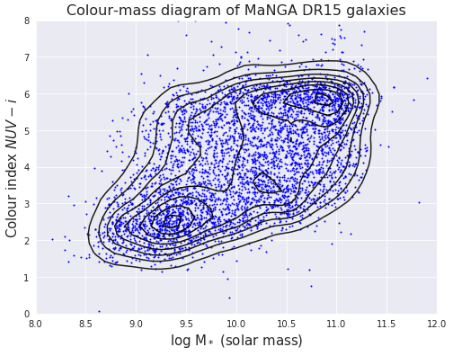
\includegraphics[width=\columnwidth]{images/CMDs/Colour-Mass-DR15-All.png}
    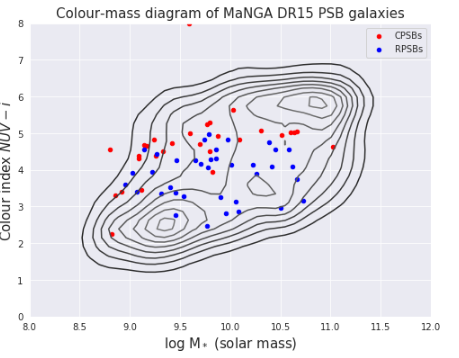
\includegraphics[width=\columnwidth]{images/CMDs/Colour-Mass-DR15-PSBs.png}
    \caption{We construct colour-mass diagrams for the full MaNGA DR15 survey population over a contour plot same this full sample (left panel). The our sample of PSBs is plotted over the same contour with the PSB galaxies plotted as points for CPSB sample (red dots) and RPSB sample (blue dots).}
    \label{fig:Colour-Mass-PSBs}
\end{figure*}


\subsection{Control galaxies}
\label{sec:controls}
A control sample set of regular galaxies not exhibiting PSB features was selected by Chen et al. (2019) sample. The purpose of the control sample is to provide a reference set of properties for comparison with the PSB data with a view to identifying typical progenitors which have not (yet) experienced a major merger. For each PSB, (CPSBs and RPSBs), a set of 10 non-PSB galaxies were selected but having similar stellar mass and global D$_n$4000 spectral indices. We used this control galaxy sample in this work.

[TODO: revise the caption in Figure \ref{fig:Colour-Mass-PSBs-controls} and ]

\begin{figure*}
    \centering
    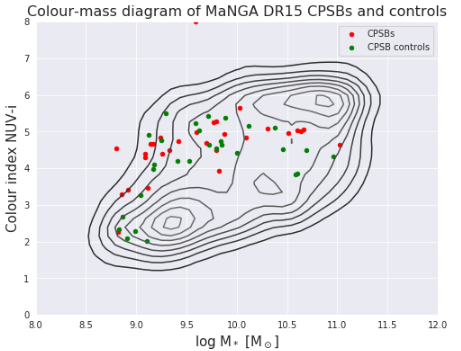
\includegraphics[width=\columnwidth]{images/CMDs/Colour-mass-CPSB+controls.png}
    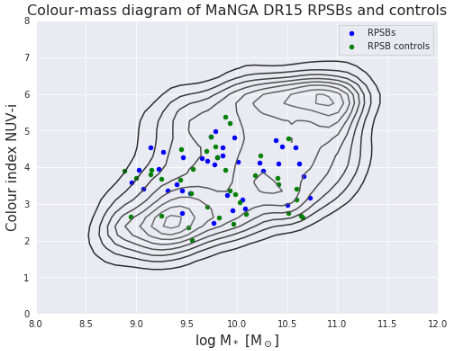
\includegraphics[width=\columnwidth]{images/CMDs/Colour-mass-RPSB+controls.png}
    \caption{Similar to Figure \ref{fig:Colour-Mass-PSBs}. The distribution of PSBs and their control galaxies has been laid over the the colour-mass contour plot of the full DR15 sample. In the left panel we have the distribution for the CPSB sample (red dots) with their control galaxies (green dots), in the right panel the RPSB sample (blue dots) with their corresponding controls (green dots).}
    \label{fig:Colour-Mass-PSBs-controls}
\end{figure*}

[TODO: add some text to highlight that the CPSBs and their controls are redward of the RPSBs.]

\subsection{PSB spectra}
The spectrum of a PSB galaxy exhibiting central PSB features is shown in Figure \ref{fig:CPSB-8623-9102-spec}.
\begin{figure*}
    \centering
    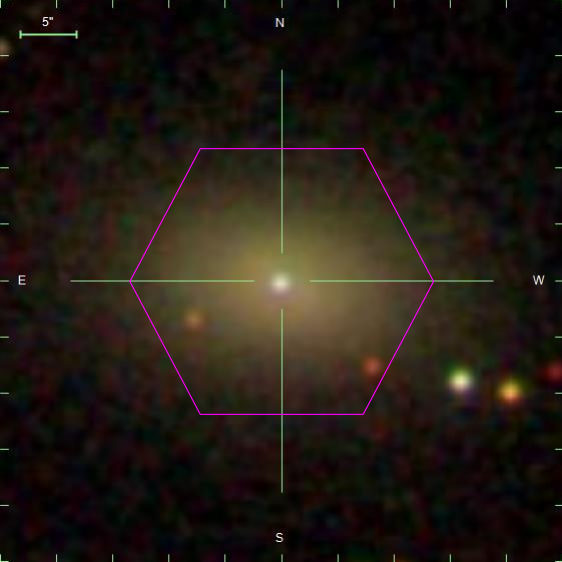
\includegraphics[width=0.22\textwidth]{images/Cutouts/CPSB-8623-9102-IM.png}
    \hfill
    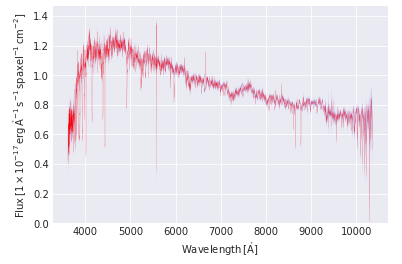
\includegraphics[width=0.38\textwidth]{images/Spectra/CPSB-8623-9102.png}
    \hfill
    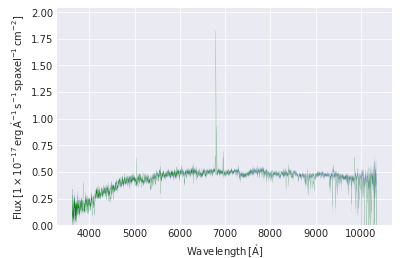
\includegraphics[width=0.38\textwidth]{images/Spectra/CPSB-CTRL-8990-3703-spec.png}
    \caption{Left: SDSS 3-colour image of central-type PSB 8623-9102. 
    Centre: The observed frame spectrum of the central spaxel of CPSB  8623-9102. Note the strong 4000 \AA\ break feature and strong hydrogen absorption lines in the wavelength region 3500 to 4500 \AA.
    Right: Observed frame spectrum of the control galaxy 8990-3703 with similar stellar mass to 8623-9102. This control galaxy shows relatively weak absorption lines and exhibits a strong H$\alpha$ emission line indicating the presence of cold gas and ongoing star formation.}
    \label{fig:CPSB-8623-9102-spec}
\end{figure*}


The spectrum of a ring-type RPSB galaxy exhibiting non-central PSB features is shown in Figure \ref{fig:RPSB-8323-6103-spec}.
\begin{figure*}
    \centering
    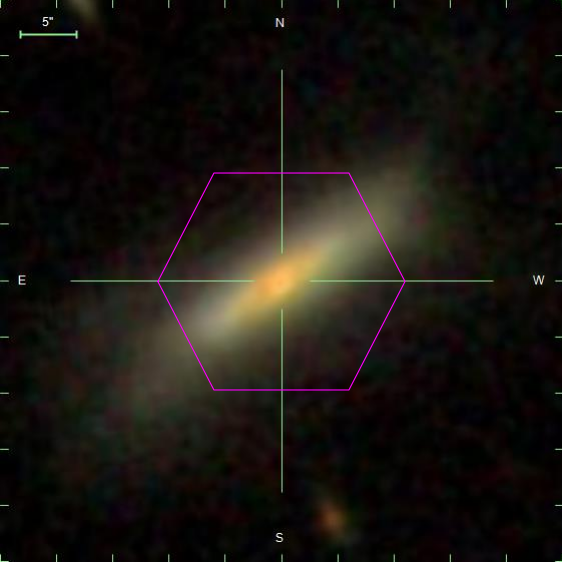
\includegraphics[width=0.24\textwidth]{images/Cutouts/RPSB-8323-6103-IM.png}
    \hfill
    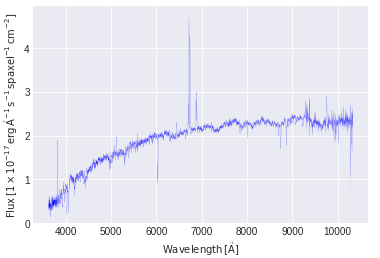
\includegraphics[width=0.35\textwidth]{images/Spectra/RPSB-8323-6103-27-27.png}
    \hfill
    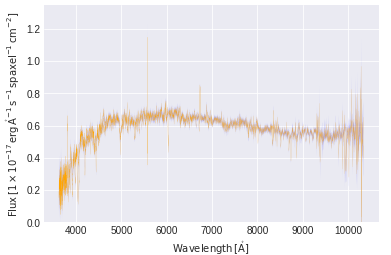
\includegraphics[width=0.35\textwidth]{images/Spectra/RPSB-8323-6103-34-32.png}
    \caption{Left: SDSS 3-colour image of the ring-type PSB 8323-6103. 
    Centre: The observed frame spectrum of the central region of ring-type PSB 8323-6103 at spaxel coordinates [27, 27] reveals strong H$\alpha$ emission consistent with an ample gas supply for continuing star formation.
    Right: The spectrum of ring-type PSB 8323-6103 at spaxel coordinates [34, 32], above and right of centre. The spectrum in this region exhibits the post-starburst features of weak emission lines, indicating a lack of gas, and strong Balmer absorption lines typical of the stellar atmospheres of A-type stars.}
    \label{fig:RPSB-8323-6103-spec}
\end{figure*}

An example of the MaNGA stellar velocity and gas velocity maps for a CPSB is illustrated in Figure \ref{fig:CPSB-8313-6101-VMAPS}.

\begin{figure}
    \centering
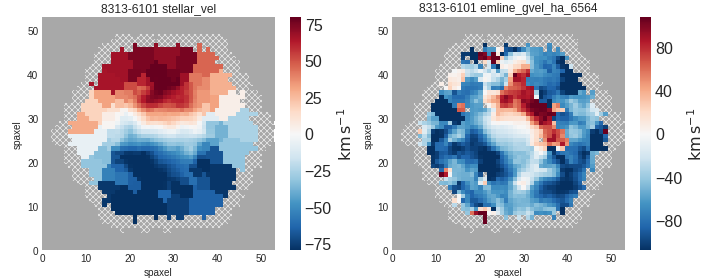
\includegraphics[width=\columnwidth]{images/VelocityMaps/CPSB-8313-6101-VMAPS.png}
    \caption{MaNGA velocity maps for CPSB 8313-6101: stellar velocity (left) and H$\alpha$ gas velocity (right).}
    \label{fig:CPSB-8313-6101-VMAPS}
\end{figure}

\subsection{Quality screening}
Global kinematic velocity position angles (PA) for the sample were determined using the \texttt{fit\_kinemetry\_pa} routine as described in appendix C of \cite{2006MNRAS.366..787K}. The routine returns the angle of the line bisecting the greatest change in velocity between the receding and approaching sides. \cite{2019MNRAS.483..172D} performed a \texttt{kinemetry} analysis of over 8,000 galaxies from the internal MPL-8 release of the MaNGA survey. In order to obtain a clean sample of well defined global PAs they visually classified the stellar and H$\alpha$ gas velocity fields of all galaxies in their sample into 3 categories (Chris Duckworth, 2019, personal communication), and set flags in their dataset as follows:

\begin{itemize}
    \item [1] Dominant coherent rotation and well defined PA. 
    \item [2] Dominant coherent rotation but with complex motions or highly inclined velocity fields 
    \item [3] Do not use
\end{itemize}

During this analysis galaxies with kinematically decoupled cores (KDCs) and warped velocity fields were also identified.

The resulting MPL-8 screened dataset from dataset of galaxies with reliable global PAs (flagged as [1] or [2]) from \cite{2019MNRAS.483..172D} was matched with the PSB galaxies in the sample of Chen et al. (2019, in prep.) to obtain a subset of PSBs with good \texttt{kinemetry} analysis flags. Furthermore a subset of those PSBs with $\Delta$PAs > 30\textdegree\ was extracted. The results are shown in Tables \ref{tab:my-CPSBs} and \ref{tab:my-RPSBs}. 

[Include a few examples of the PDF output from kinemetry: Chris' plots.]

In classical Kinemetry analysis it is considered significant if the $\Delta$PA position angle is greater than 30 degrees. We show some examples of misaligned stellar and gas velocity fields here: 
[TODO: tidy up this section.]

\begin{figure}
    \centering
    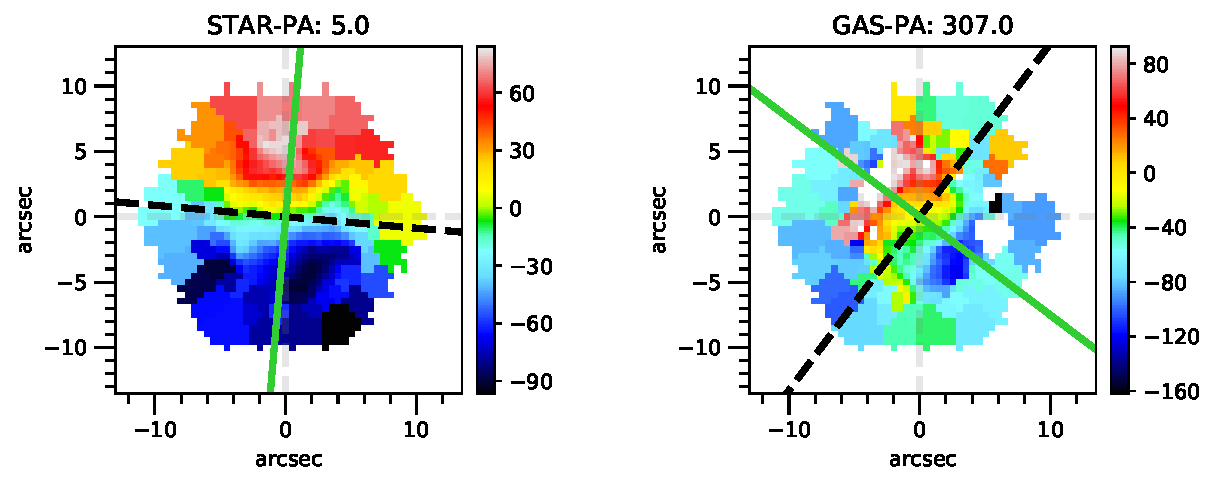
\includegraphics[width=\columnwidth]{images/PAplots/PAplotsCPSB/8313-6101-PA.pdf}
    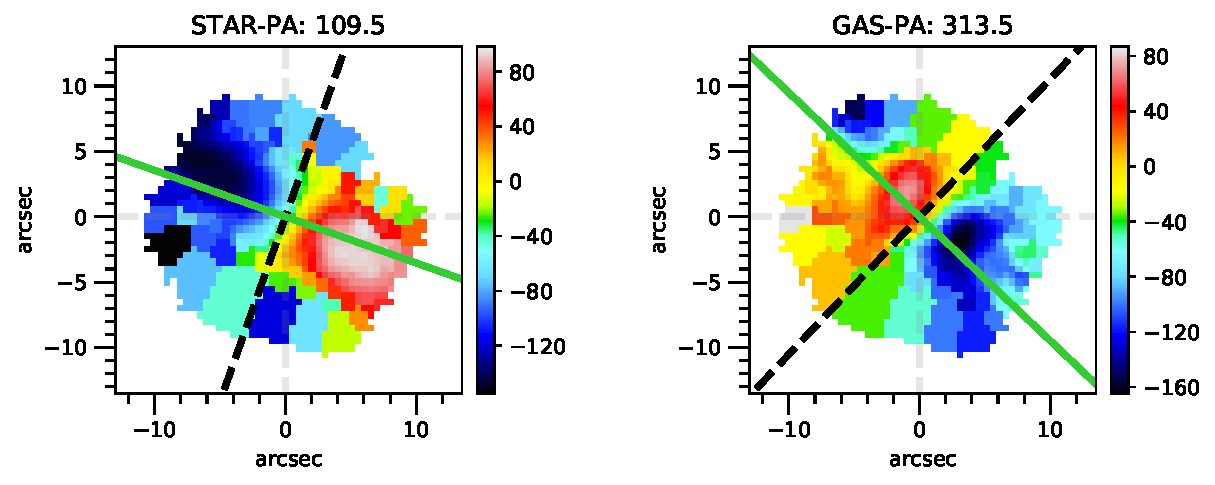
\includegraphics[width=\columnwidth]{images/PAplots/PAplotsRPSB/8323-6103-PA.pdf}
    \caption{Kinemetry-derived position angles (PA) for stellar velocity (left) and gas velocity (right) of two PSB galaxies exhibiting a significant $\Delta$PA. Top: CPSB 8313-6101, and bottom: RPSB 8323-6103. The velocity position angle is displayed as the green solid line while the black dashed line denotes the bisector of the velocity field between the receding (red) and blue (approaching) sides. The velocity colour scale is \kms. Credit for data analysis and plots: Chris Duckworth}
    \label{fig:CPSB-8313-6101-PA}
\end{figure}

\begin{table}
\caption{CPSBs with PA offset \textgreater 30 deg.}
\label{tab:offsetCPSBs}
\begin{tabular}{lccc}
\hline
PlateIFU  & Stellar PA & H$\alpha$ PA & $\Delta$PA \\
  & (deg.) & (deg.) & (deg.) \\
\hline
8313-6101 & 5 & 307 & 58 \\
8655-1902 & 335 & 127 & 152 \\
8725-1902 & 22 & 175 & 153 \\
8938-6102 & 214 & 47.5 & 166.5 \\
9494-3701 & 140.5 & 243 & 102.5 \\
\hline
\end{tabular}
\end{table}

\subsection{PA plots: misaligned RPSBs}

\begin{table}
\caption{RPSBs with PA offset \textgreater 30 deg.}
\label{tab:offsetRPSBs}
\begin{tabular}{lccc}
\hline
PlateIFU   & Stellar PA & H$\alpha$ PA & $\Delta$PA \\
  & (deg.) & (deg.) & (deg.) \\
\hline
8080-3704 & 24 & 154 & 130 \\
8262-3701 & 153.5 & 118.5 & 35 \\
8323-6103 & 109.5 & 313.5 & 156 \\
8439-6104 & 5.5 & 107 & 101.5 \\
8453-3704 & 44 & 91 & 47 \\
8486-1901 & 295.5 & 85 & 149.5 \\
8554-3701 & 250 & 68 & 178 \\
8932-12704 & 166.5 & 134.5 & 32 \\
9872-3701 & 208.5 & 81 & 127.5 \\
\hline
\end{tabular}
\end{table}

